\documentclass[final, 16pt]{beamer}
% poster
\usepackage[size=custom, width=101.6, height=71.1]{beamerposter}
% common stuff
\usepackage{graphicx}
\usepackage{hyperref}
\usepackage{booktabs}
\usepackage{amsmath}
\usepackage{caption}
\usepackage{subcaption}
\usepackage{enumitem}
\usepackage{array}
\usepackage{xparse}
\usepackage{wrapfig}
\usepackage{xspace}
% necessary acronyms
\def\ie{\textit{i.e.}\xspace}
\def\eg{\textit{e.g.}\xspace}
\def\etc{\textit{etc.}\xspace}
\def\etal{\textit{et al.}\xspace}
\def\cf{\textit{cf.}\xspace}
% font
\usefonttheme{serif}
\setbeamerfont{block title}{size=\Large, series=\bfseries}
\setbeamerfont{headline title}{size=\fontsize{64}{0pt}\selectfont, series=\bfseries}
\setbeamerfont{headline author}{size=\large, series=\bfseries}
% main color
\definecolor{theme-1}{HTML}{10b981} % #10b981
\definecolor{theme-2}{HTML}{14b8a6} % #14b8a6
\definecolor{theme-3}{HTML}{f5f5f4} % #f5f5f4
\definecolor{theme-4}{HTML}{fafaf9} % #fafaf9
% set color
\setbeamercolor{block title}{fg=theme-3, bg=theme-1}
\setbeamercolor{headline title}{fg=theme-4, fg=theme-1}
% linespace
\usepackage{setspace}
\setstretch{1.25}
% size
\setlength{\paperwidth}{40in}
\setlength{\paperheight}{28in}
\newlength{\sepwidth}
\newlength{\colwidth}
\newlength{\twocolwidth}
\newlength{\contentwidth}
\newlength{\contentheight}
\newlength{\marginwidth}

\usepackage{calc}
\setlength{\marginwidth}{0.5in}
\setlength{\contentwidth}{\paperwidth - 2\marginwidth}
\setlength{\contentheight}{\paperheight - 3in}
\setlength{\sepwidth}{0.005\contentwidth}
% 4 columns
\setlength{\colwidth}{(\contentwidth - 3\sepwidth) / 4}
\setlength{\twocolwidth}{\colwidth + \sepwidth + \colwidth}
% empty spacer column
\NewDocumentCommand{\separatorcolumn}{}{\begin{column}{\sepwidth}\end{column}}
\NewDocumentCommand{\margincolumn}{}{\begin{column}{\marginwidth}\end{column}}
% top head template
\setbeamertemplate{headline}{
  \begin{beamercolorbox}{headline}
    \usebeamerfont{headline}
    \vskip1.5in
    \centering
    {\usebeamerfont{headline title}\usebeamercolor[fg]{headline title}\inserttitle\\[0.5ex]}
    {\usebeamerfont{headline author}\usebeamercolor[fg]{headline author}\insertauthor\\[1ex]} % author is not allowed.
    \ifbeamercolorempty[bg]{headline rule}{}{
      \begin{beamercolorbox}[wd=\paperwidth,colsep=0.5ex]{headline rule}\end{beamercolorbox}
    }
  \end{beamercolorbox}
}
\usepackage{tikz}
\usetikzlibrary{calc}
\NewDocumentCommand{\ensuremargin}{}{
  \begin{tikzpicture}[remember picture,overlay]
    \draw[black] ($(current page.north west) - (0, 1.5in)$) -- ($(current page.north east) - (0, 1.5in)$);
    \draw[black] ($(current page.south west) + (0, 1.5in)$) -- ($(current page.south east) + (0, 1.5in)$);
    \draw[black] ($(current page.north west) + (1in, 0)$) -- ($(current page.south west) + (1in, 0)$);
    \draw[black] ($(current page.north east) - (1in, 0)$) -- ($(current page.south east) - (1in, 0)$);
  \end{tikzpicture}
}
% header helper
\usepackage{xhfill}
\NewDocumentCommand{\header}{m O{1.5em}}{\vspace{#2}\begingroup\usebeamercolor[bg]{block title}\scshape\large#1\par\vspace{-0.55\baselineskip}\hrulefill\endgroup}
\NewDocumentCommand{\subheader}{m}{\begingroup\usebeamercolor[bg]{block title}\bfseries#1\par\endgroup}

% multicol
\usepackage{multicol}
% hanging indent
\usepackage{hanging}
% numbered figure and table
\setbeamertemplate{caption}[numbered]
% metadata
\title{Wireless Online Real-time Language Expression Yielder}
\author{Ian Oberbeck \& Yubo Cao \& Anish Goyal \\\normalfont GOSA Governor's Honors Program 60 Engineering}
% bullet
\setlist[itemize]{leftmargin=0.5em, label=\usebeamercolor[bg]{block title}\textbullet}
% redefine block
\let\block=\undefined
\let\endblock=\undefined
\usepackage[most]{tcolorbox}
\newtcolorbox{block}[1]{enhanced, colback=white, colframe=theme-1!50, colbacktitle=theme-1, coltitle=white, fonttitle=\bfseries, title=\Large#1, boxrule=1pt, boxsep=1.5em, breakable, sharpish corners, bottomrule=0.5em, toptitle=-0.75em, bottomtitle=-0.75em}
% microtype
\usepackage[activate={true,nocompatibility},final]{microtype}

% remove navigation
\setbeamertemplate{navigation symbols}{}
% make vfill work in beamer columns
\usepackage{etoolbox}
\let\oldcolumn\column
\let\oldendcolumn\endcolumn
\RenewDocumentEnvironment{column}{m O{\contentheight - 2.7in}}{%
  \oldcolumn{#1}%
  \minipage[c][#2][s]{\columnwidth}
}{\endminipage\oldendcolumn}

\begin{document}

\begin{frame}[t]
\centering
\begin{columns}[t]
\margincolumn

\fontsize{22}{26}\selectfont

\begin{column}{\colwidth}
  \fontsize{22}{24}\selectfont
  \begin{block}{Background}
    \header{Goal}[0pt]

    The goal of \textsc{Project Worley} is to create a wireless online real-time language expression yielder (WORLEY) that can be used to act out American Sign Language (ASL) live. Specifically, WORLEY will be able to:

    \begin{itemize}
      \item Recognize speech and translate it into ASL in real time.
      \item Act out the translation on the robotic hand through remote general-purpose input/output (GPIO) control.
    \end{itemize}

    \header{Motivation}[0pt]

    Our friend Cory suffers from hearing loss, making communication difficult. We aimed to develop a device to improve communication and quality of life for Cory and others in similar situations.

    This device can also be used for Pre-K and K-12 students.  While it may seem easy for parents to learn ASL and teach it to their kids, ASL is a complex language with its own grammar, syntax, and nuances. WORLEY provides the necessary language exposure \& support for hard-of-hearing children and their parents.
  \end{block}

  \begin{figure}
    \centering
    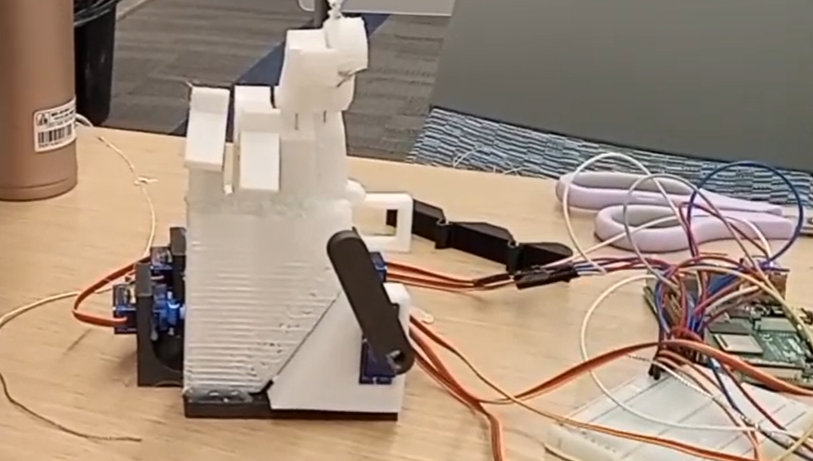
\includegraphics[width=0.75\linewidth]{images/hand.png}
    \caption{WORLEY's robotic hand.}
    \label{fig:hand}
  \end{figure}

  \begin{block}{Introduction}

    One of the key distinguishing features of this project is its real-time interpretation capability. Unlike existing systems that require a delay between input and output, our team developed a solution that could instantaneously translate spoken words into sign language. 

    Moreover, we designed WORLEY with the grammar and syntax of ASL in mind. ASL gloss is a shortened representation of traditional English with its own distinct syntax and grammar. Using transformers, WORLEY can translate spoken English into ASL gloss, which is then converted into ASL signs.

    Another significant aspect of WORLEY lies in the design of the robotic hand. The hand does not have a reset stage between frames, which optimizes the signing process. Additionally, we designed an efficient rotation scheme for the thumb that reduced the DoF by 2, reducing the cost of the project and making it more accessible. 

    % To accomplish the project goals, the team employed a multidisciplinary approach, combining knowledge and skills from various engineering fields such as robotics, signal processing, and machine learning. The team members worked collaboratively, leveraging their diverse expertise to tackle different aspects of the project.

    % In conclusion, the Final Engineering Project for the 60th Georgia Governor's Honor Program aimed to develop a unique system that could convert voice input into ASL output in real-time. By focusing on real-time interpretation, ASL grammar, and a signing-optimized hand design, the project sought to overcome existing limitations in the field. The endeavor required innovation, technical expertise, and collaboration, ultimately aiming to provide a valuable tool for both presentations and the teaching of sign language.
  \end{block}

\end{column}

\separatorcolumn

\begin{column}{\twocolwidth}
  \begin{block}{Significance}
    \begin{minipage}[t]{0.48\linewidth}
      \header{Existing Solution}[0pt]
    \begin{figure}[ht]
      \centering
      \begin{subfigure}[b]{0.38\linewidth}
        \centering
        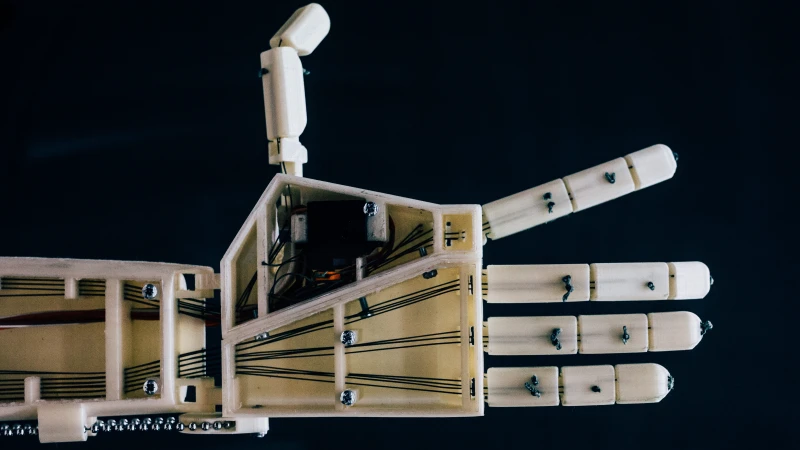
\includegraphics[width=\linewidth]{images/aslan.png}
        \caption{Project ASLAN}
        \label{fig:aslan}
      \end{subfigure}
      \begin{subfigure}[b]{0.38\linewidth}
        \centering
        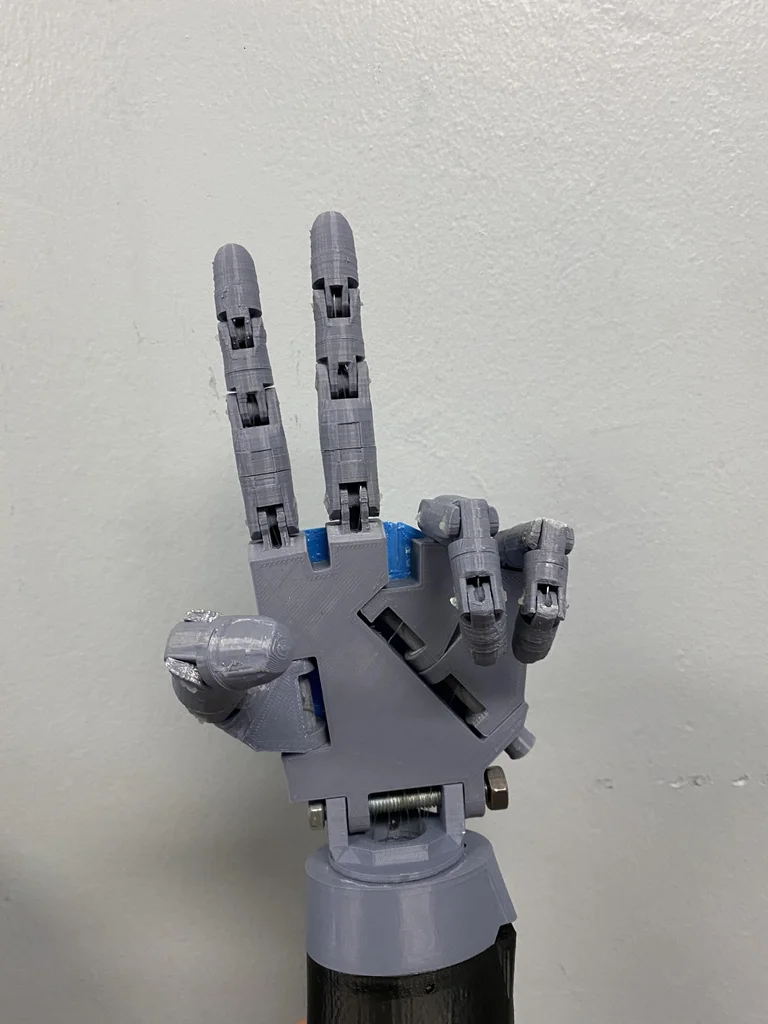
\includegraphics[width=0.425\linewidth]{images/instructable-hand.png}
        \caption{Instructable Hand}
        \label{fig:instructable-hand}
      \end{subfigure}
    \end{figure}
    \vspace{-1em}
    
    Despite the existing solutions, there are still many problems:
    
    \begin{itemize}
      \item They merely perform manually-coded English (MCE).
      \item They are incapable to act out ASL in real-time and require text input.
    \end{itemize}
    \end{minipage}\hfill%
    \begin{minipage}[t]{0.48\linewidth}
      \header{Significance}[0pt]

      \begin{itemize}
        % \item 10,000 people in the United States are registered as ASL interpreters.
        \item In comparison, 37.5 million people in the United States suffer from hearing problems.
        % \item ASL is the third most used language in the United States \& the Americans with Disabilities Act (ADA) requires businesses to provide ASL interpreters.
        \item In the United States, 30 deaf children are born every day, and 90\% of their parents do not know ASL.
        \item \emph{WORLEY} will help to solve this problem by providing a low-cost, portable, and easy-to-use solution for ASL interpretation.
      \end{itemize}
    \end{minipage}
    
  
  \end{block}

  \begin{block}{System Architeture}
    \begin{minipage}{0.48\linewidth}
      \begin{figure}[ht]
        \centering
        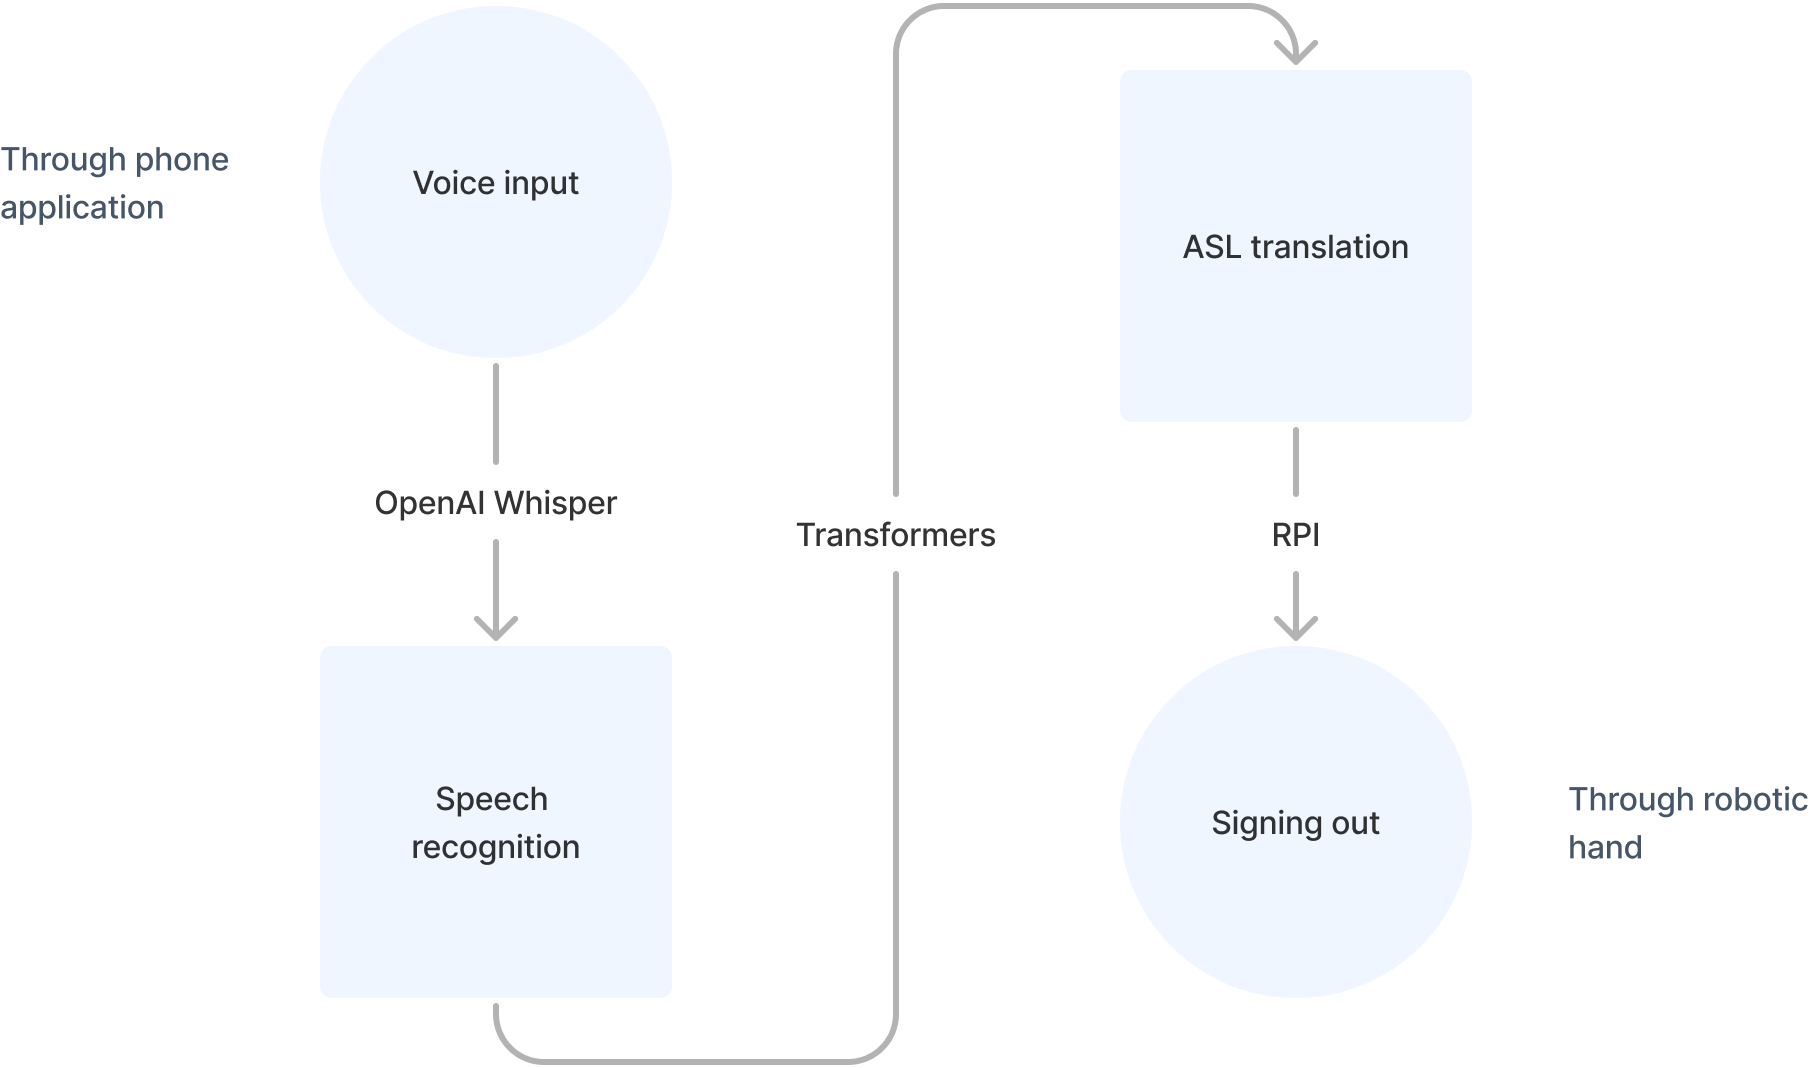
\includegraphics[width=\linewidth]{images/flowchart.png}
        \caption{Flowchart of the system architecture}
        \label{fig:flowchart}
      \end{figure}
    \end{minipage}\hfill%
    \begin{minipage}{0.48\linewidth}
      \begin{itemize}
        \item The user speaks into the Worley application on their phone.
        \item The application establishes a Web real-time communication (WebRTC) connection with the server and streams the audio.
        \item The server runs a lightweight voice activation detection (VAD) model \texttt{sliero} detects speech. Such results are buffered into a queue along with the timestamps, and a 2-pointer technique is used to extract the longest continuous subsequence, \ie, the speech. Such segments are sent to \texttt{whisper} for speech recognition.
        \item The text is translated to ASL language using a custom-built transformer model trained on the \texttt{ASLG-PC12} dataset.
        \item The ASL translation is sent to the Raspberry Pi, which controls the robotic hand, and the mobile application.
      \end{itemize}
    \end{minipage}
  \end{block}

  \begin{block}{Mechanical Design}
    \begin{minipage}[t]{0.48\linewidth}
      \header{Cord Actuation}[0pt]

      \begin{wrapfigure}{r}{0.30\linewidth}
        \centering
        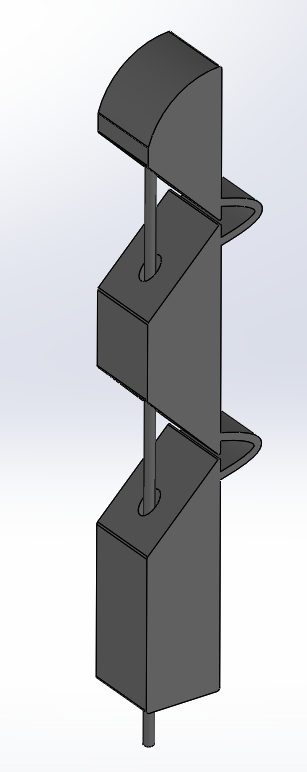
\includegraphics[width=0.35\linewidth]{images/finger.png}
        \caption{CAD of cord actuation design}
        \label{fig:cord-actuation}
      \end{wrapfigure}

      The fingers are curled by servo-driven pull cords. By reducing the available length of the cord, the surfaces of the finger segments are pulled closer to one another. The surfaces are angled 90 degrees; so the finger rotates around the back (where there is no gap) to curl. We utilized ripoff SG90 servos for this task, as they're cost-effective, space-efficient, and have the minimum sufficient torque required to actuate the fingers.
    \end{minipage}\hfill%
    \begin{minipage}[t]{0.48\linewidth}
      \header{Compliant Hinges}[0pt]

      \begin{wrapfigure}{r}{0.30\linewidth}
        \centering
        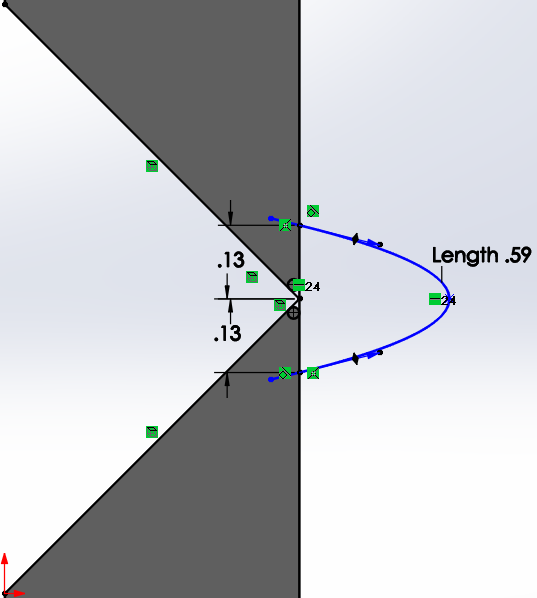
\includegraphics[width=0.75\linewidth]{images/compliant-hinge.png}
        \caption{CAD of compliant hinge design}
        \label{fig:compliant-hinge}
      \end{wrapfigure}

      Compliant hinges connect the finger segments, allowing the finger to curl as a single part. This is accomplished by 3D printing the fingers in polypropylene (PP); a polymer ideally suited for compliant hinges due to its fatigue-resistant and semi-rigid properties. The hinges are designed using splines constrained by their connection points and length, such that when the segment is rotated 90 degrees it has the proper length to temporarily deform into a circle. The energy stored in this deformation allows the fingers to passively return to their original position when the cord tension is released.
    \end{minipage}
  \end{block}
\end{column}

\separatorcolumn

\begin{column}{\colwidth}
  \fontsize{22}{24}\selectfont
  \begin{block}{Challenges}
    \begin{itemize}
      \item More tolerance would be needed for the servo motors to control the index finger to move behind the palm.
      \item Whisper model, even the CTranslate2 version, would require $1735\,\text{ms}\pm 139\,\text{ms}$ to translate a 3-second speech, which is not real-time. Deployment of the servo independently from the HTTP server on KServe would be needed to ensure performance and scalability.
      \item Polypropylene failed to print successfully on the 3D printer; further, the printed version has structural defects \& fatigue issues, rendering the hand to be less realistic.
    \end{itemize}
  \end{block}

  \begin{block}{Material}
    \begin{itemize}
      \item 5 SG90 servo, servo horns, and screws
      \item 4 3D printed fingers + 1 3D printed palm
      \item Polypropylene filament \& Polylactic acid filament
      \item 1 Raspberry PI 4B
      \item \texttt{faster\_whisper}, \texttt{pytorch}, \texttt{asyncio}, \texttt{pyav}, \texttt{aiohttp}, \texttt{aiortc}, Expo Framework.
    \end{itemize}
  \end{block}
  \begin{block}{Conclusion}
    \header{Future Work}[0pt]

    Despite WORLEY's current limitations, we believe it has the potential to be further developed and improved. Future work could implement the following:
    
    \begin{description}
      \item[Speaker diarization] The current implementation cannot distinguish between multiple speakers.
      \item[Advanced model deployment] The current implementation is not \emph{truly} real-time, since the model is not deployed independently from the HTTP server.
      \item[Enhance realism] We want to make the hand more realistic. This can be done by adding ball joints to the thumb and wrist. We could also add a layer of silicone to simulate skin.
      \item[Wire management] To make the hand more aesthetically pleasing, we will position the servos inside of a compartment in the upper arm, and run the wires through the arm to the hand.
    \end{description}
    
    \header{Result}[0pt]

    Remarkably, WORLEY came to life in a mere nine days and a budget of just 150 USD. Moving forward, our aspirations lie in crafting a comprehensive prototype given ample time and resources. We triumph in knowing we successfully developed a robotic hand that can act out the ASL alphabet and be controlled using a mobile application with automatic speech recognition.

  \end{block}
\end{column}

\margincolumn
\end{columns}

\tikz {
  \draw ($(current page.south west)!0.5!(current page.south east)$) node {All charts, graphs, photos, and diagrams are the product of the student researcher.};
}
\end{frame}
\end{document}

